\documentclass{article}

\usepackage{amsmath}
\usepackage{amssymb}	
\usepackage{graphicx}
\usepackage{float}
\newcommand{\HRule}{\rule{\linewidth}{0.5mm}}
\setlength{\parindent}{0in}
\setlength{\parskip}{12pt}
\usepackage[margin=1.0in]{geometry}
\usepackage{algorithm}
\usepackage{algpseudocode}

\usepackage{listings}
\usepackage{xcolor}
\lstset { %
    language=C++,
    backgroundcolor=\color{black!5}, % set backgroundcolor
    basicstyle=\footnotesize,% basic font setting
}

\definecolor{codegreen}{rgb}{0,0.6,0}
\definecolor{codegray}{rgb}{0.5,0.5,0.5}
\definecolor{codepurple}{rgb}{0.58,0,0.82}
\definecolor{codeblue}{rgb}{0,0.4,1}
\definecolor{backcolour}{rgb}{0.95,0.95,0.92}

\lstdefinestyle{mystyle}{
	language=C++,
    backgroundcolor=\color{backcolour},   
    commentstyle=\color{codegreen},
    keywordstyle=\color{codeblue},
    numberstyle=\tiny\color{codegray},
    stringstyle=\color{codepurple},
    basicstyle=\ttfamily\footnotesize,
    breakatwhitespace=false,         
    breaklines=true,                 
    captionpos=b,                    
    keepspaces=true,                 
    numbersep=5pt,                  
    showspaces=false,                
    showstringspaces=false,
    showtabs=false,                  
    tabsize=2
}

\lstset{style=mystyle}


\begin{document}

\begin{titlepage}
\begin{center}

\textsc{\LARGE University of Queensland}\\[1.5cm]
\textsc{\Large COSC7502 Major Project - Milestone 2}\\[0.5cm]

\HRule \\[0.4cm]
{\huge \bfseries Genetic Algorithm\\[0.4cm]}
\HRule \\[1.5cm]

\begin{minipage}{0.4\textwidth}
\begin{flushleft} \large
\textbf{Name}\\
Tristan Burns
\end{flushleft}
\end{minipage}
\begin{minipage}{0.4\textwidth}
\begin{flushright} \large
\textbf{Student Number} \\
42648493
\end{flushright}
\end{minipage}



\vfill

{\large \today}

\end{center}

\end{titlepage}



\section{Summary}
\begin{abstract}
This report details the serial implementation, verification and performance optimisation of solution to the OneMax problem using a Genetic Algorithm implemented in C++.
\end{abstract}
This report details the serial implementation, verification and performance optimisation of solution to the OneMax problem using a Genetic Algorithm implemented in C++. 

\section{Serial Implementation} 
\subsection{Algorithm} 
The genetic algorithm is a type of metaheuristic optimisation algorithm which has biologically inspired iterative crossover and mutation of candidate solutions. 

Pseudo-code for the algorithm implemented in this project is presented in  Algorithm 1. 

\begin{algorithm}
\caption{The Genetic Algorithm}\label{alg:cap}
\begin{algorithmic}

\State $n \gets $ Chromosome Size
\State $m \gets $ Population Size
\State $p \gets \lbrace\rbrace$ \Comment{Population of \(m\) individuals with chromosomes of length \(n\)} 
\State $q \gets \lbrace\rbrace$ \Comment{Children of \(m\) individuals with chromosomes of length \(n\)} 
\State $maxgenerations \gets $ Max generations.
\State $best \gets $ null
\State $generation \gets 0$ 
\State $fitness \gets \lbrace\rbrace$ 
\For{\(m\) times}
	\State $p \gets$ random individual \Comment{Define a random seed to permit deterministic behaviour}
\EndFor
\While{$best \neq n$ \textbf{and} $generations < maxgenerations$ }
\For{each $i$ in $p$}
	\State $fitness[i] \gets IndividualFitness(i)$
\EndFor
\State $best$ = max($fitness$)
\For{$m/2$ times }
\State Parents $p_1, p_2\gets select(p)$ \Comment{Use tournament selection in this implementation}
\State Children $c_1, c_2\gets crossover(p)$ \Comment{Use single point crossover in this implementation}
\State  $q\gets \lbrace mutate(c_1),mutate(c_1)\rbrace$ \Comment{Use bitflip mutation in this implementation}
\EndFor
\State  $p\gets q$
\State $generation++$
\EndWhile \\
\Return $best$
\end{algorithmic}
\end{algorithm}

There are many possible variations on the genetic algorithm. Key features of this implementation are summarised as comments in Algorithm 1.


\subsection{OneMax Problem}
The OneMax problem is defined as the maximum number of value 1 bits in a bit string. Solution of the OneMax problem is effectively searching for a bitsting of exclusively ones. 

For the Genetic Algorithm this is encoded in the chromosome, with possible genes of 0 or 1. In this implementation, a Genetic Algorithm is used to search through a population of \(m\) individuals with chromosomes of length \(n\) for a chromosome consisting of only ones. In this case a fitness function is defined to be the sum of all chromosomes, with optimal fitness being equal to the chromosome sum \(n\).

\subsection{Program Implementation}
The genetic algorithm was implemented in C++ and compiled to C++11 standard using g++. Optimisation flags are discussed in Section 4.3 below.

The program is structured to use of macros for user defined constants and static arrays with memory allocated at compile time. In order to maximise performance, verbose functions were duplicates of the non-verbose counterparts, to avoid passing verbose arguments with subsequent internal branching. 

\section{Verification}
The implementation was verified through explicit inspection of verbose output results and plotting the (normalised fitness over time) for a number of trials. An advantage of the OneMax problem is that the optimal solution and associated fitness is the same as the chromosome size \(n\), permitting easy verification.  Because of the stochastic nature of genetic algorithms a  random seed was defined as an input parameter to enable deterministic and repeatable results.

Verbose output allowed for explicit verification of the key steps of the Genetic Algorithm, namely computing fitness, \textit{crossover} and \textit{mutation} verification. See Annex A for a single loop of verbose output.


\begin{figure}[H]
\centering
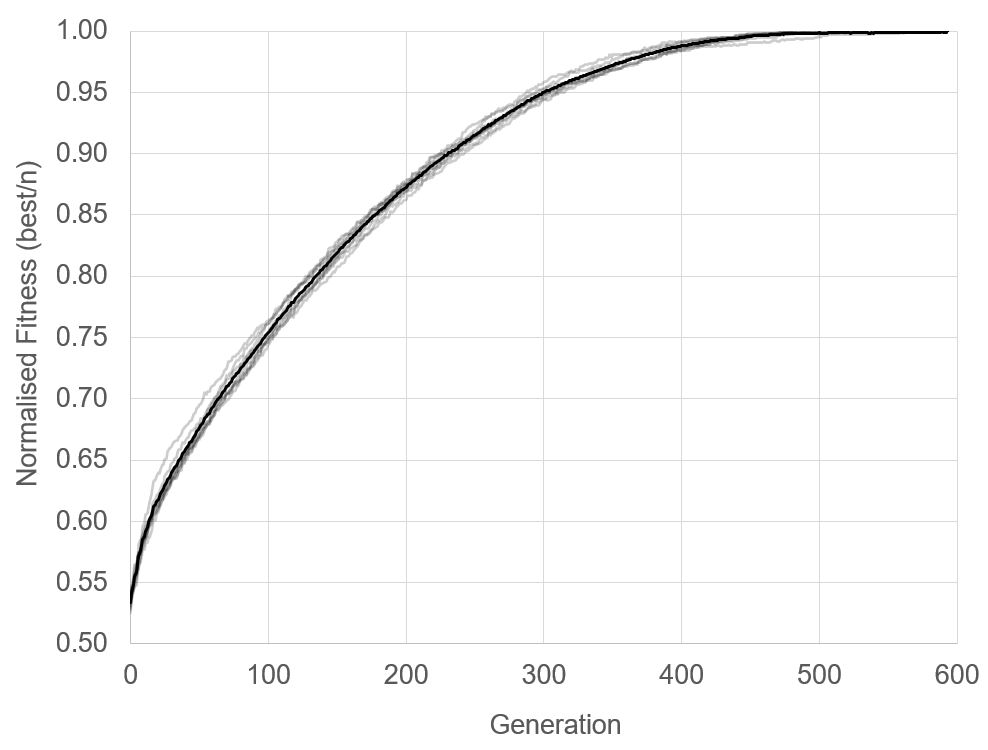
\includegraphics[scale=0.6]{normfit.png}
\caption{Normalised fitness vs number of generations, \(n\), for a population size of \(m=100\) and a chromosome size of \(n=1024\). Different random seeds where used (light grey results), with the average  plotted in black, demonstrating robust convergence for large problem size.}
\end{figure}

\newpage
\section{Performance Optimisation}

\subsection{Manual Optimisation}
An attempt was made to manually optimise the code based on gprof profiling. The program was compiled with the \textit{-pg -O0} flags set. Based on gprof profiling (see Annex B), the function \textit{Mutate} (see below), was identifed as taking approximately 21 percent of the runtime. 
\begin{lstlisting}
void Mutate(int *q, int n, int m)
{
    int mu;
    for (int i = 0; i < m; i++)
    {
        for (int j = 0; j < n; j++)
        {
            mu = (std::rand() % n);
            if (mu == 0)
            {
                (q(i, j)) = 1 - (q(i, j));
            }
        }

    }
    return;
}
\end{lstlisting}
An attempt was made to remove the internal branching as follows. 
\begin{lstlisting}
void Mutate(int *q, int n, int m)
{
    int mu;
    for (int i = 0; i < m; i++)
    {
        
        for (int j = 0; j < n; j++)
        {
            mu = ((std::rand() % n)==0);
            q(i, j) = (q(i, j))*(1-mu) + (1 - (q(i, j)))*(mu); //remove branching
        }

    }
    return;
}
\end{lstlisting}
However, followup profiling revealed that this actually made performance worse with the function \textit{Mutate} taking approximately 37 percent of the runtime. Therefore, this implementation was reverted and optimisation was focused on compile flags, as discussed in section 4.2


\subsection{Optimisation Flags}
Because of the number of nested loops in the \textit{Crossover}, \textit{Assess Individual fitness} and \textit{Mutate}, it was inferred that -funroll-loops would yield improvements.

What was unexpected, was the flags -flto and -fuse-linker-plugin in combination yielding a ~10-20 percent improvement on -O3 optimisation alone.  Although I do not  understand this improvement from the documentation, I hypothesise that these flags improve the optimization by exposing more code to the link-time optimizer. 

\subsection{Performance Results}
\begin{figure}[H]
\centering
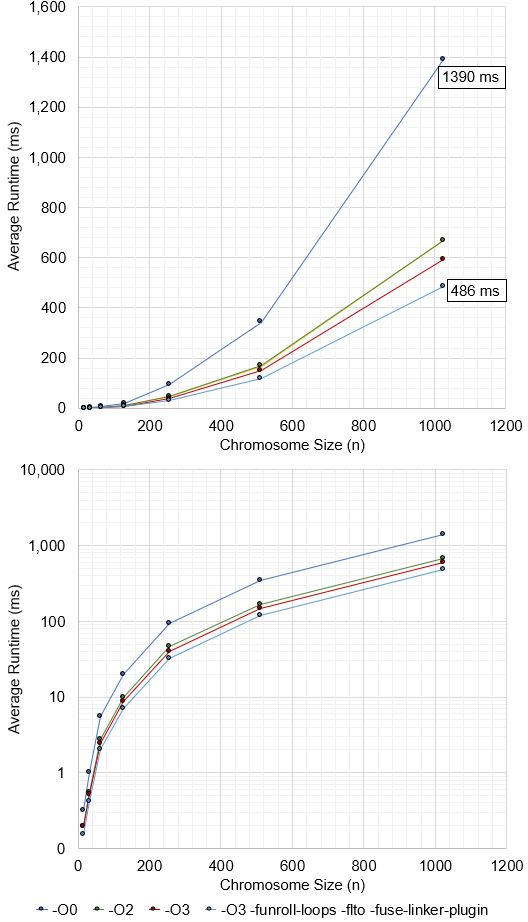
\includegraphics[scale=0.85]{avruntime2.png}
	\caption{Average runtime (ten trials) vs chromosome size, \(n\), for a population size of \(m=100\) individuals. Based on different optimisation flags a \(\sim 2.8\times\) speedup is achieved. These results were computed using the same random seed, \textit{seed }\(=42\).}
\end{figure}

next sec
Random communication patterns are difficult to implement in MPI. MPI is based on all ranks having a deterministic set of communication patterns.


\newpage



\bibliography{coscbibdemo} 
\bibliographystyle{ieeetr}

\newpage
\section*{Annex A - Verbose Example}
Using the following inputs, the verbose output for a single loop is displayed as an example.
\begin{lstlisting}
#define n 16                  // Chromosome size (number of genes per individual).
#define m 8                   // Population size (number of individuals).
#define seed 42               // Psuedorandom number generator seed (std:srand(seed)).
#define maxgenerations 2000   // Maximum number of generations (while loop limit).
#define t 2                   // Tournament size (parents competing for selection).
#define verbose true          // Verbose output (cout) for verification.
#define printfitness false    // Best fitness per generation output (cout).
\end{lstlisting}
Single loop (generation) verbose output (cout):
\begin{lstlisting}
Running MaxFitness (Verbose)
0011001011011000 -> Individual 0, Fitness: 7
0001101111101011 -> Individual 1, Fitness: 10
0000011011101111 -> Individual 2, Fitness: 9
0101010111101110 -> Individual 3, Fitness: 10
1100010101010110 -> Individual 4, Fitness: 8
0110111001000101 -> Individual 5, Fitness: 8
0010010000011111 -> Individual 6, Fitness: 7
0101011101100100 -> Individual 7, Fitness: 8
 ------------ Generation: 0 Best Fitness: 10 --------------
Running Crossover (Verbose)
Crossover at chromosome 7:
0001101|111101011 -> Parent 1 (Individual 1)
0110111|001000101 -> Parent 2 (Individual 5)
0001101|001000101 -> Child 0
0110111|111101011 -> Child 1
Crossover at chromosome 7:
0110111|001000101 -> Parent 1 (Individual 5)
1100010|101010110 -> Parent 2 (Individual 4)
0110111|101010110 -> Child 2
1100010|101000101 -> Child 3
Crossover at chromosome 15:
000110111110101|1 -> Parent 1 (Individual 1)
010101011110111|0 -> Parent 2 (Individual 3)
000110111110101|0 -> Child 4
010101011110111|1 -> Child 5
Crossover at chromosome 0:
|0001101111101011 -> Parent 1 (Individual 1)
|0001101111101011 -> Parent 2 (Individual 1)
|0001101111101011 -> Child 6
|0001101111101011 -> Child 7
Running Mutate (Verbose)
 0  0  0  1  1  0  1 *1* 0  1  0  0  0 *0* 0  1 -> Child 0 Mutation at *_* 
 0  1  1  0  1  1  1  1  1  1  1  0  1  0  1  1 
 0  1  1  0  1  1  1  1 *1* 1  0  1  0  1  1  0 -> Child 2 Mutation at *_* 
 1 *0* 0  0  0  1  0  0  0  1 *1* 0  0  1  0  1 -> Child 3 Mutation at *_* 
 0  0  0  1  1  0 *0* 1  1  1  1  0  1  0  1  0 -> Child 4 Mutation at *_* 
 0  1  0  1  0  1  0  1  1  1  1  0  1  1  1  1 
 0  0  0  1  1  0  1  1  1  1  1  0  1  0  1  1 
 0  0  0  1  1  0  1  1  1  1  1  0  1  0  1  1 
Assigning next generation (Verbose)
0001101101000001 -> Child 0 to Individual 0, Fitness: 6
0110111111101011 -> Child 1 to Individual 1, Fitness: 12
0110111111010110 -> Child 2 to Individual 2, Fitness: 11
1000010001100101 -> Child 3 to Individual 3, Fitness: 6
0001100111101010 -> Child 4 to Individual 4, Fitness: 8
0101010111101111 -> Child 5 to Individual 5, Fitness: 11
0001101111101011 -> Child 6 to Individual 6, Fitness: 10
0001101111101011 -> Child 7 to Individual 7, Fitness: 10
\end{lstlisting}


\section*{Annex B - Profiling Results}

Initial gprof results, prior to (attempted) manual optimisation of the function \textit{Mutate}.
\begin{lstlisting}
Each sample counts as 0.01 seconds.
  %   cumulative   self              self     total           
 time   seconds   seconds    calls  ms/call  ms/call  name    
 38.19      0.45     0.45   144600     0.00     0.00  IndividualFitness(int, int*, int, int)
 21.21      0.70     0.25      482     0.52     0.52  Mutate(int*, int, int)
 17.82      0.91     0.21      482     0.44     0.44  NextGeneration(int*, int*, int, int)
 11.88      1.05     0.14      483     0.29     0.29  MaxFitness(int*, int, int)
 10.18      1.17     0.12      482     0.25     1.20  Crossover(int, int*, int*, int, int)
  0.85      1.18     0.01    48200     0.00     0.01  TournamentSelection(int, int*, int, int)
  0.00      1.18     0.00        1     0.00     0.00  _GLOBAL__sub_I__Z14ParseArgumentsiPPc
  0.00      1.18     0.00        1     0.00     0.00  _GLOBAL__sub_I_useseed
  0.00      1.18     0.00        1     0.00     0.00  PrintFitness(int*, int)
  0.00      1.18     0.00        1     0.00     0.00  RandomPopulation(int*, int, int)
  0.00      1.18     0.00        1     0.00     0.00  __static_initialization_and_destruction_0(int, int)
  0.00      1.18     0.00        1     0.00     0.00  __static_initialization_and_destruction_0(int, int)
\end{lstlisting}
gprof results, after to (attempted) manual optimisation of the function \textit{Mutate}. Subsequently, the initial implmentation of mutate was used. 
\begin{lstlisting}
Each sample counts as 0.01 seconds.
  %   cumulative   self              self     total           
 time   seconds   seconds    calls  ms/call  ms/call  name    
 37.98      0.55     0.55      482     1.14     1.14  Mutate(int*, int, int)
 27.62      0.95     0.40   144600     0.00     0.00  IndividualFitness(int, int*, int, int)
 12.43      1.13     0.18      482     0.37     1.20  Crossover(int, int*, int*, int, int)
 10.36      1.28     0.15      483     0.31     0.31  MaxFitness(int*, int, int)
  8.98      1.41     0.13      482     0.27     0.27  NextGeneration(int*, int*, int, int)
  0.00      1.41     0.00    48200     0.00     0.01  TournamentSelection(int, int*, int, int)
  0.00      1.41     0.00        1     0.00     0.00  _GLOBAL__sub_I__Z14ParseArgumentsiPPc
  0.00      1.41     0.00        1     0.00     0.00  _GLOBAL__sub_I_useseed
  0.00      1.41     0.00        1     0.00     0.00  PrintFitness(int*, int)
  0.00      1.41     0.00        1     0.00     0.00  RandomPopulation(int*, int, int)
  0.00      1.41     0.00        1     0.00     0.00  __static_initialization_and_destruction_0(int, int)
  0.00      1.41     0.00        1     0.00     0.00  __static_initialization_and_destruction_0(int, int)
\end{lstlisting}




\end{document}


\begin{lstlisting}
int** p = new int*[m];
for(int i = 0; i < m; ++i)
{
	p[i] = new int[n];
}
\end{lstlisting}


\begin{center}
\begin{tabular}{|l|cccc|}
\hline
Processors	&1		&2		&4		&8 \\
\hline
Runtime (s) 	&1400 &900  &600  &500\\
\hline
\end{tabular}
\end{center}

\begin{center}
\begin{figure}[h]
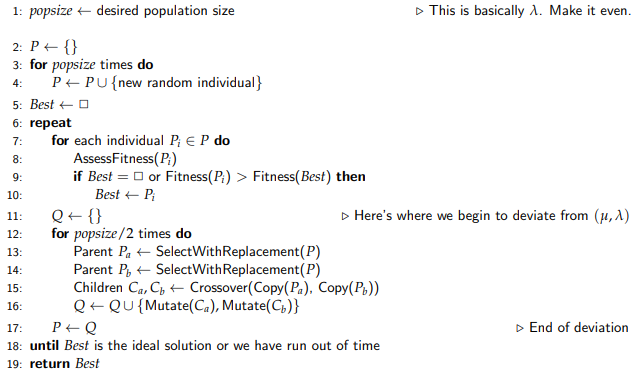
\includegraphics[scale=0.5]{genalg.png}
	\caption{Average runtime (ten trials) vs chromosome size, \(n\), for a population size of \(m=100\) individuals. Based on different optimisation flags a \(\sim 3\times\) speedup is achieved. These results were computed using the same random seed, \textit{seed }\(=42\).}
\end{figure}
\end{center}